% \begin{figure}[!ht]
%     \centering
%     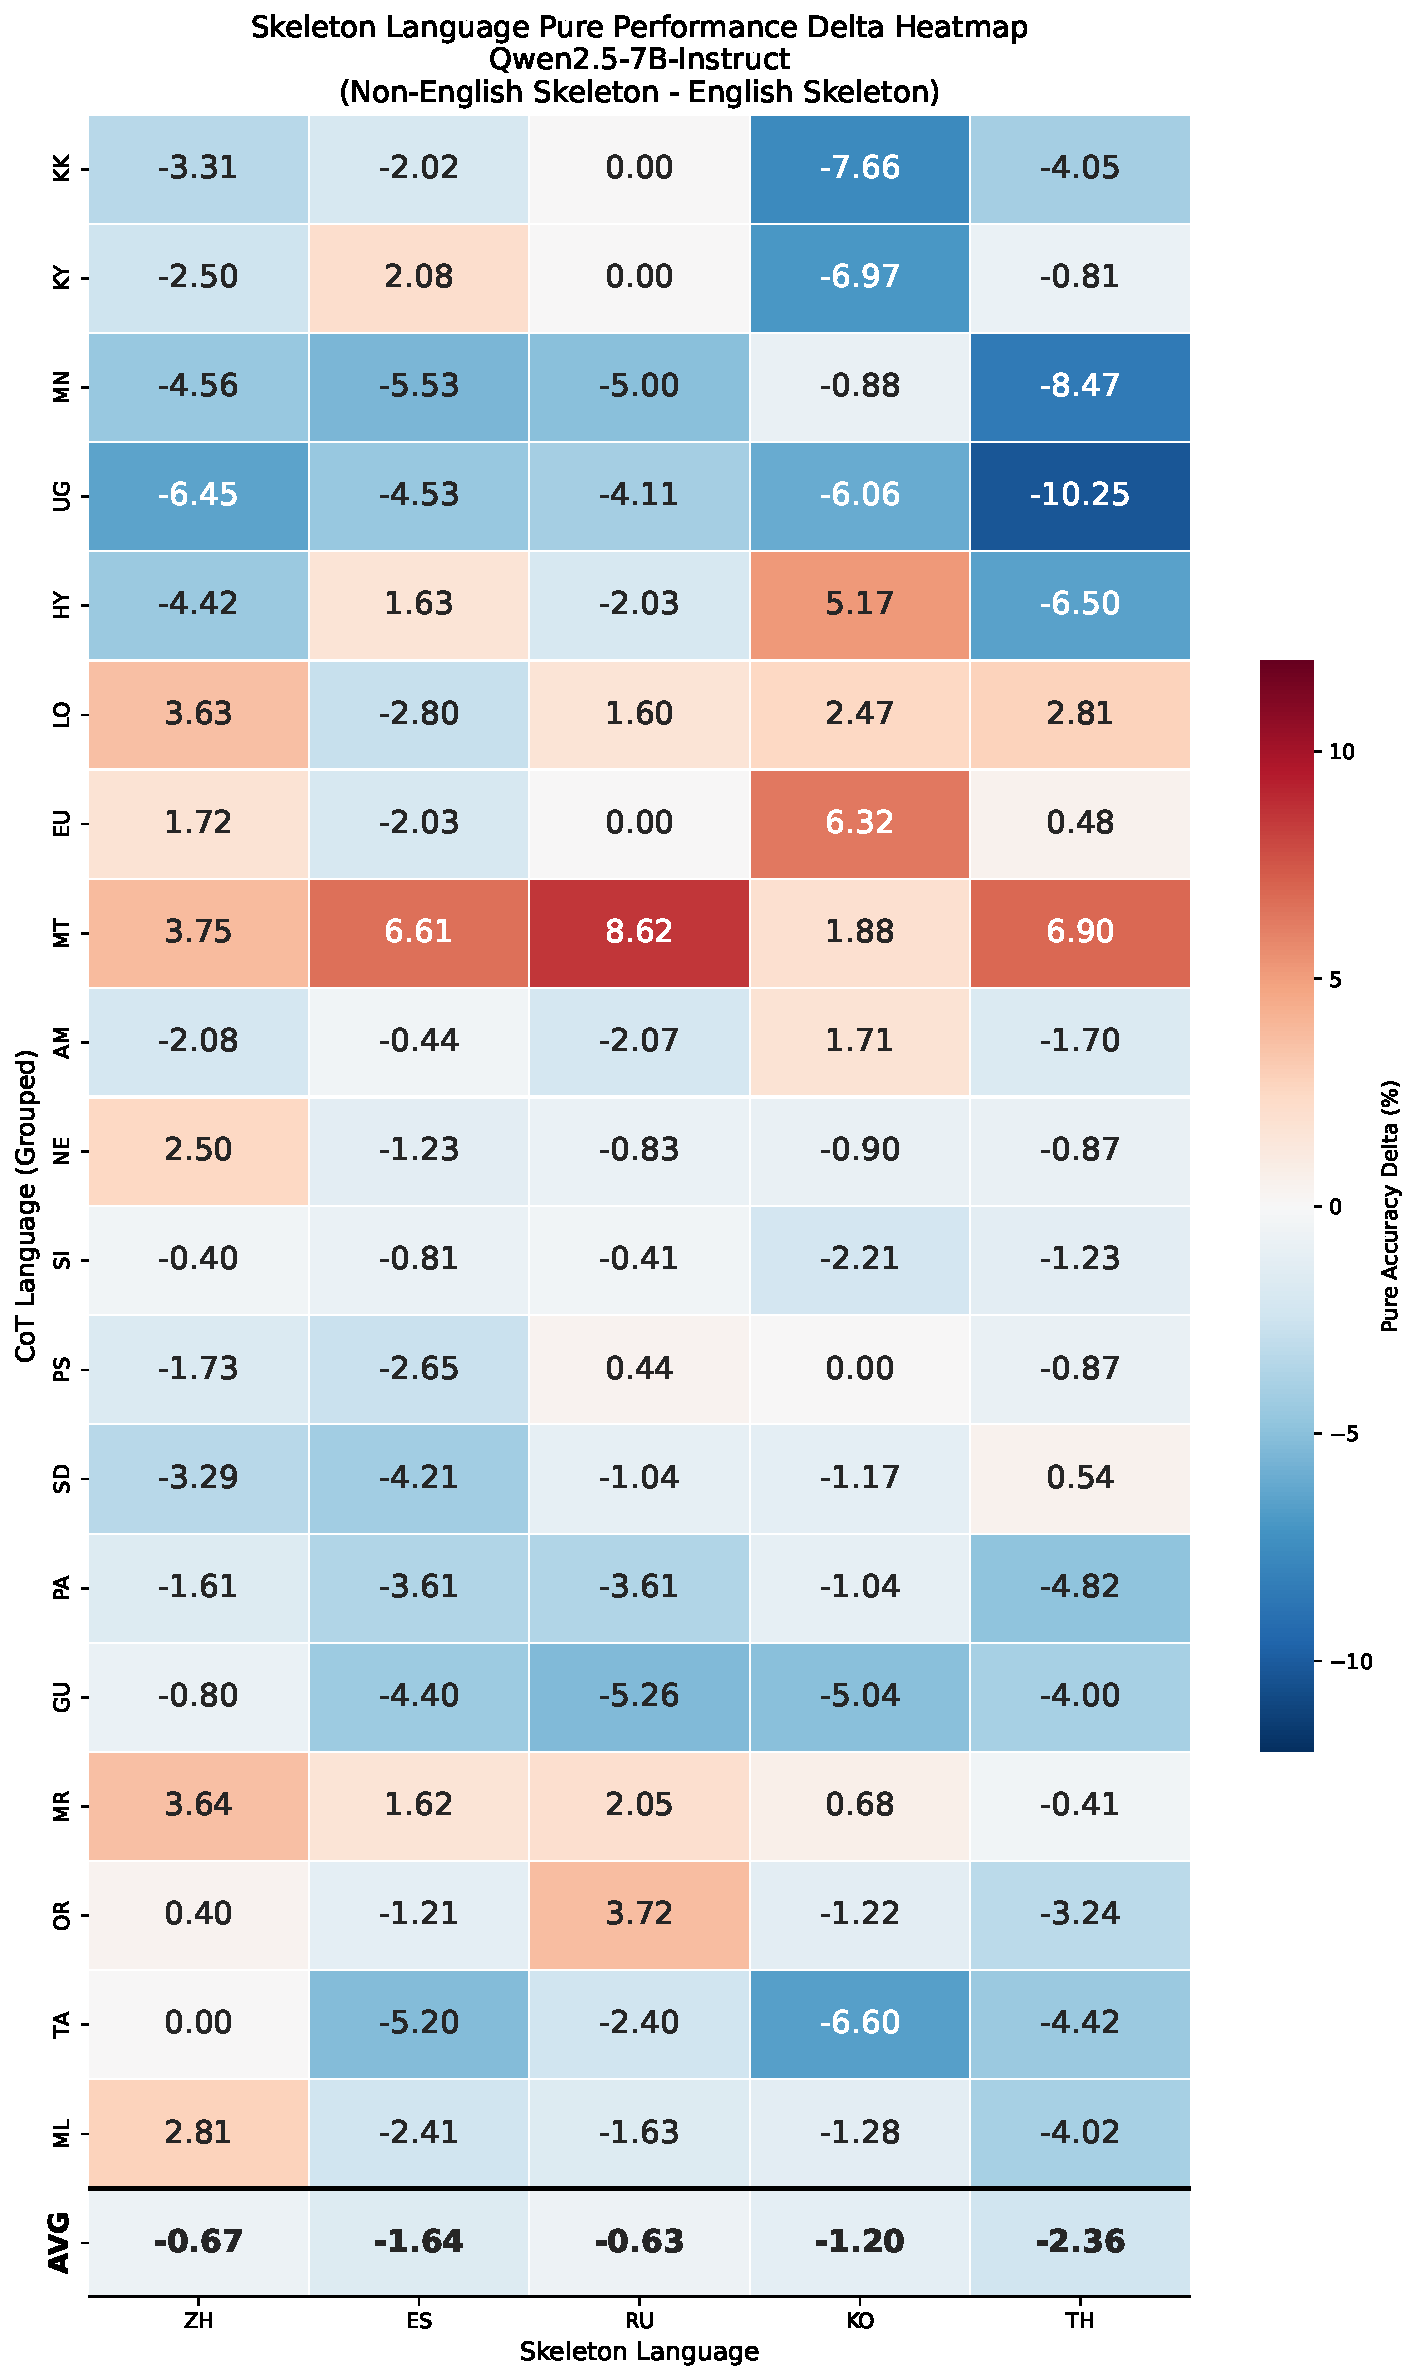
\includegraphics[width=\linewidth]{Figures/Images/Qwen2.5-7B-Instruct_single_pure_delta_heatmap_sorted.pdf}
%     \caption{\small Performance differences (Non-English $-$ English) on the MGSM under the CoT-$\ell_t$ setting with \textsc{Qwen2.5-7B}. English skeleton is replaced with five Non-English skeletons (ZH, ES, RU, KO, and TH). While English generally provides a stable default skeleton language, several target languages exhibit gains with specific Non-English skeletons, indicating that skeleton effectiveness is language-dependent.}
%     \label{fig:cross-lingual-skeleton}
%     \vspace{-0.15in}
% \end{figure}

\begin{figure*}[!ht]
    \centering
    \captionsetup[subfigure]{labelformat=simple, labelsep=space}
    \renewcommand\thesubfigure{(\alph{subfigure})}
    \begin{subfigure}[t]{0.48\linewidth}
        \centering
        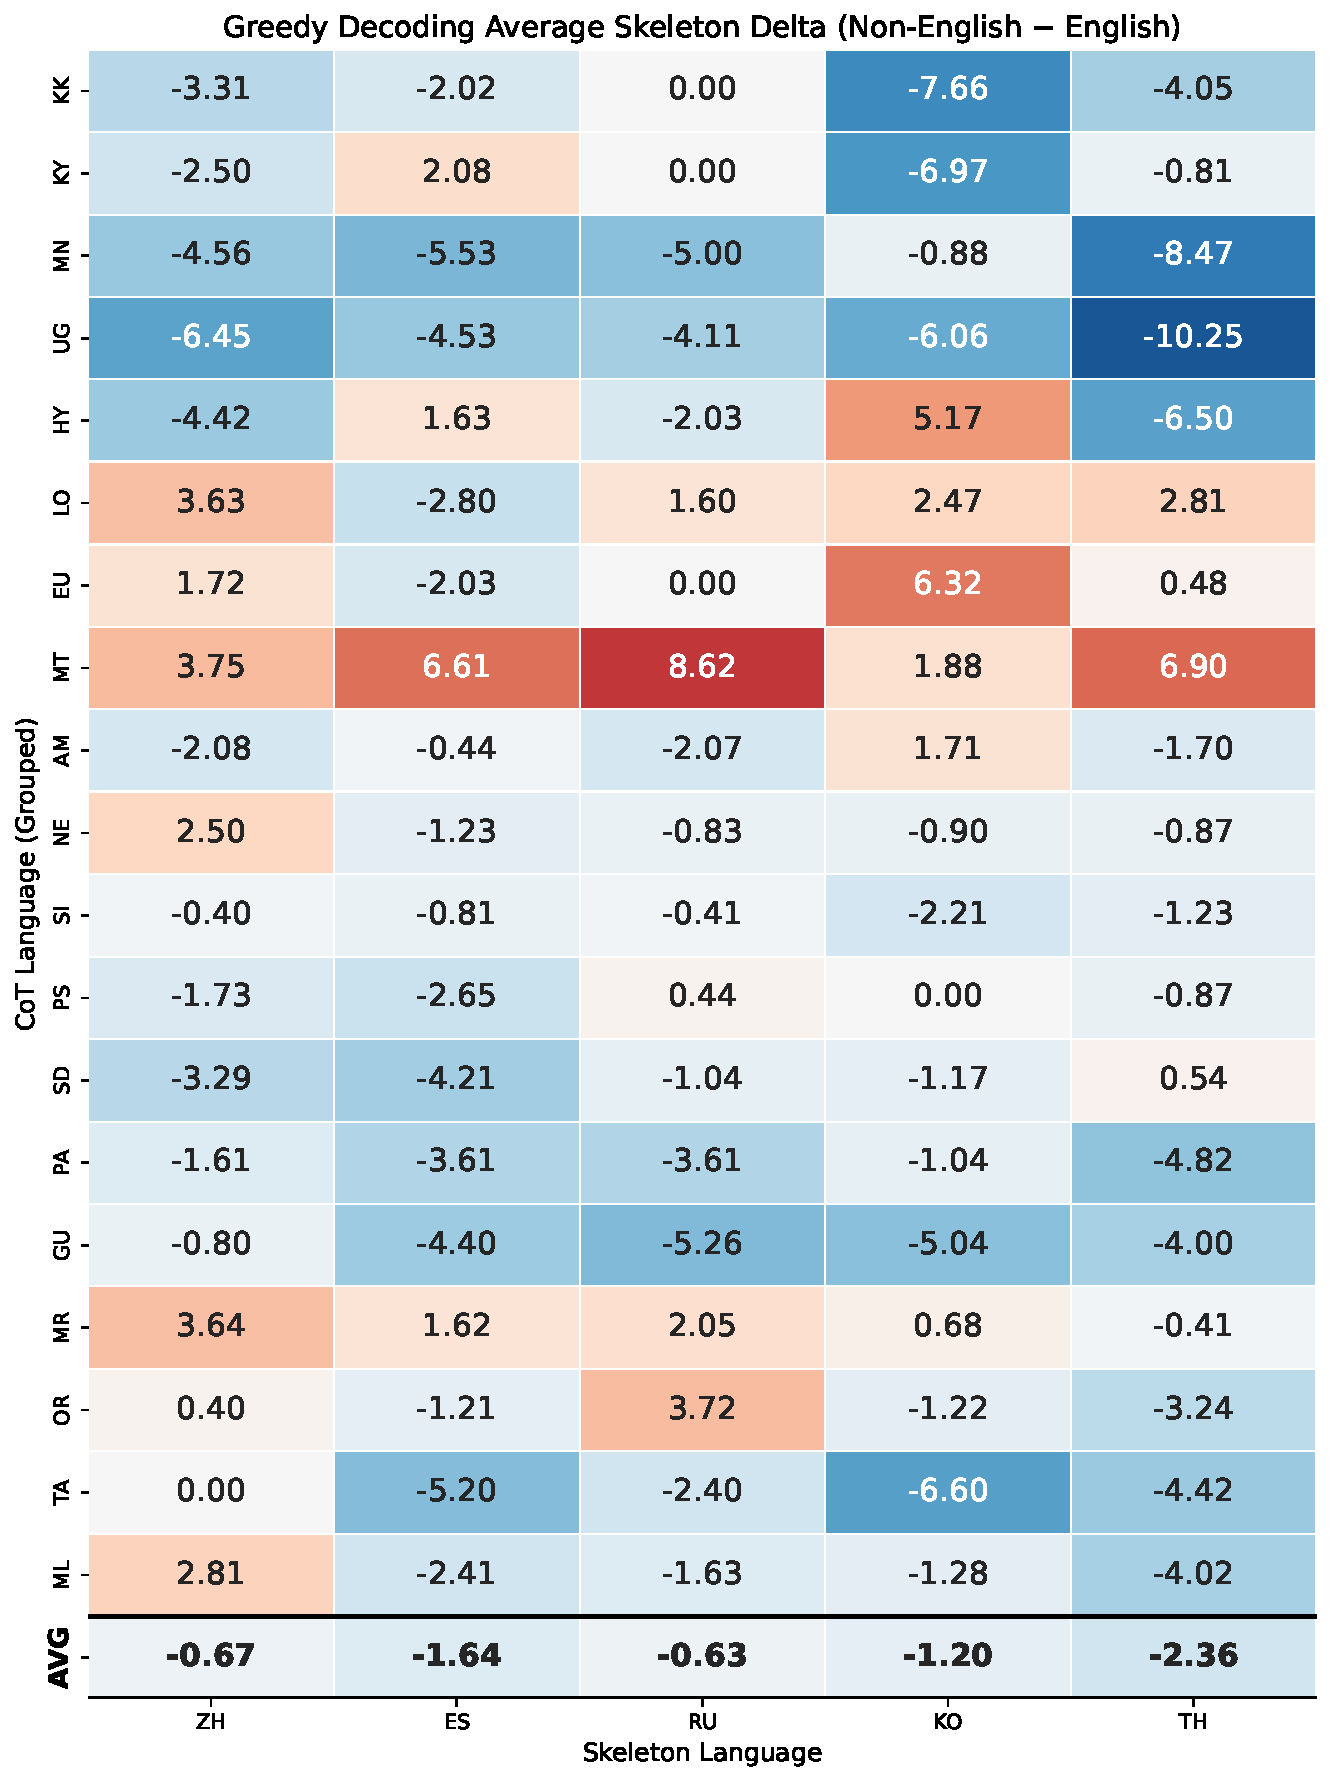
\includegraphics[width=\linewidth]{Figures/Images/greedy.pdf}
        \caption{Greedy Decoding (single rollout)}
        \label{fig:heatmap-greedy}
    \end{subfigure}
    \hfill
    \begin{subfigure}[t]{0.48\linewidth}
        \centering
        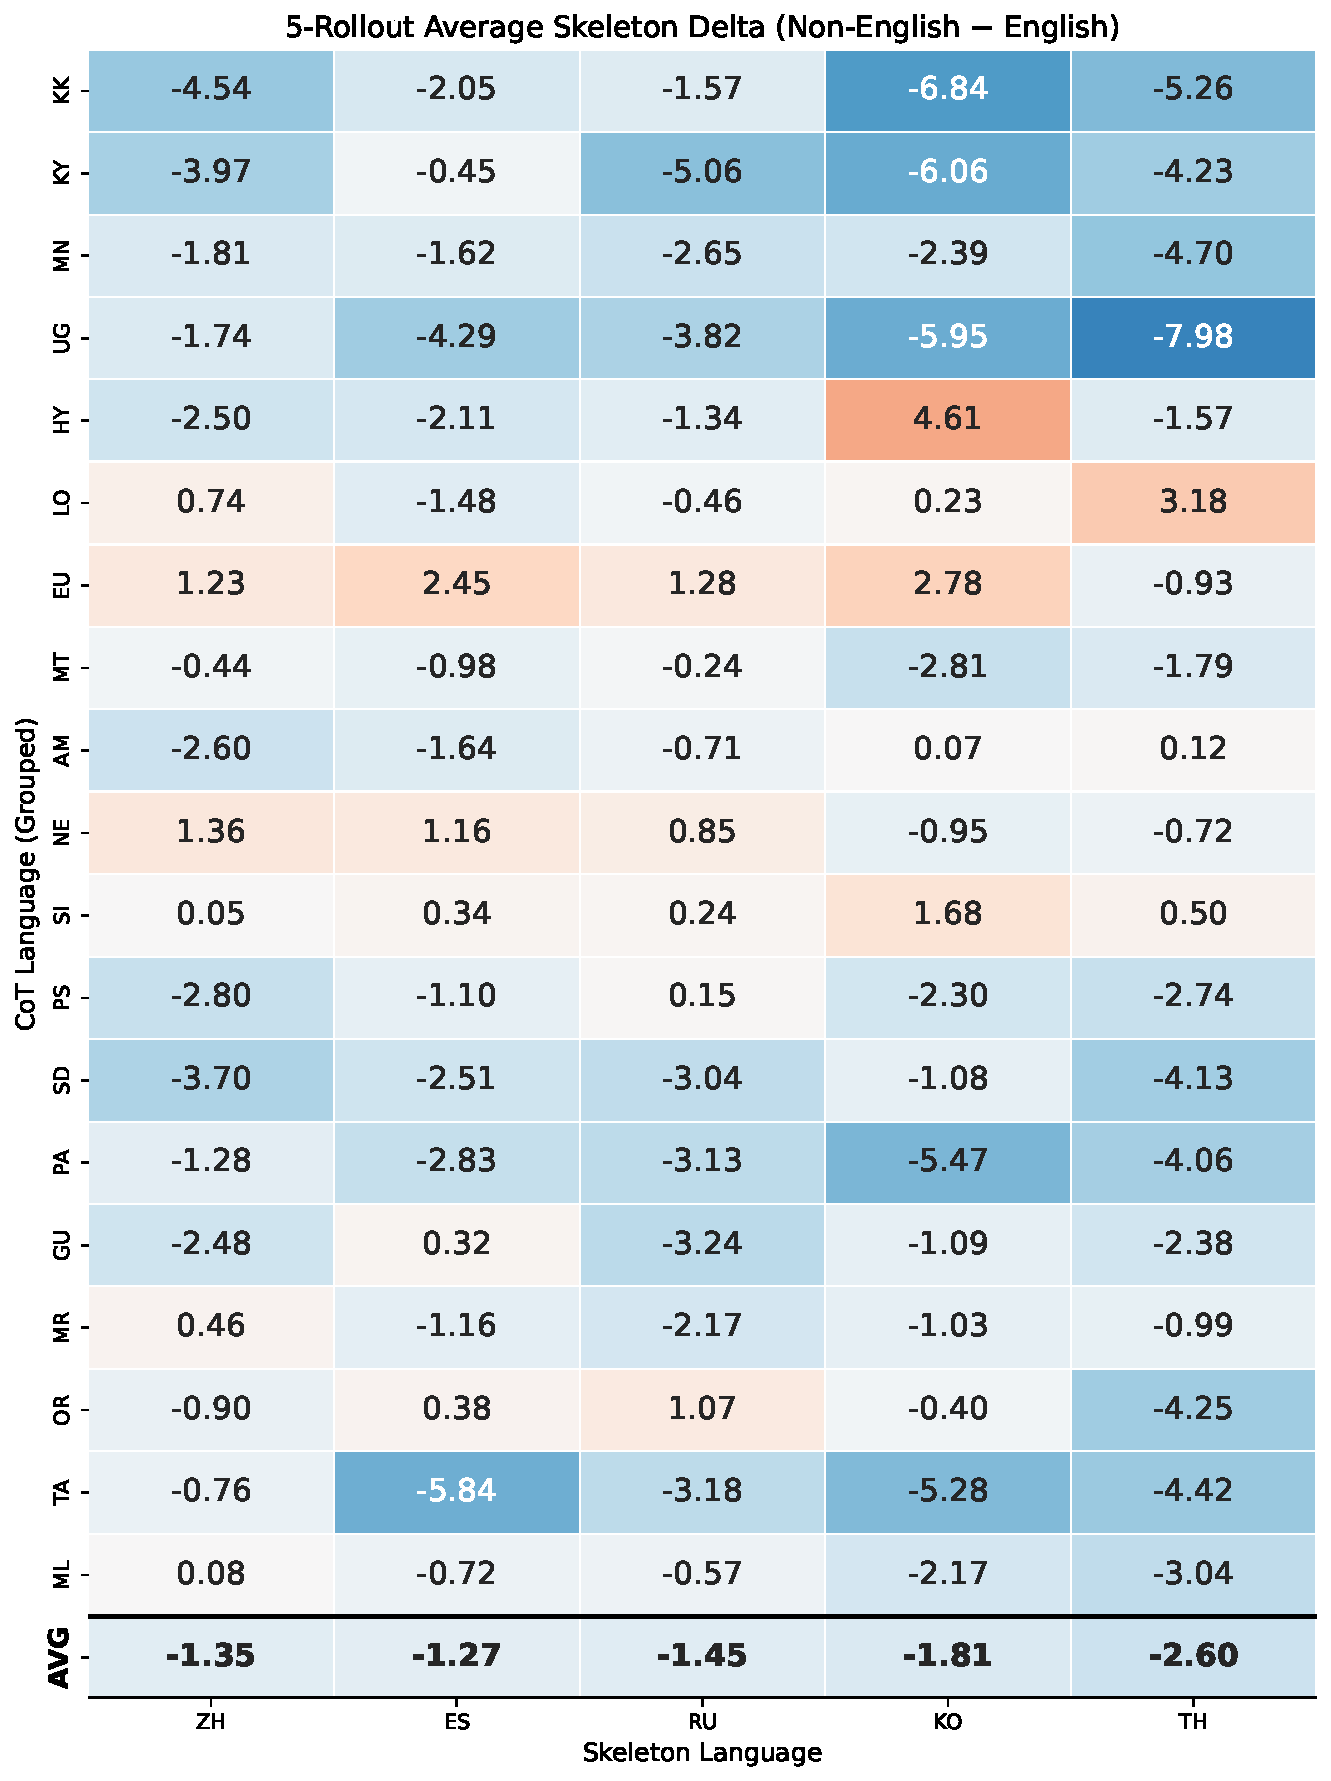
\includegraphics[width=\linewidth]{Figures/Images/5rollout.pdf}
        \caption{Multi-rollout ($T{=}0.7$, $N{=}5$)}
        \label{fig:heatmap-rollout5}
    \end{subfigure}
    \caption{\small Performance differences (Non-English $-$ English) on MGSM under CoT-$\ell_t$ with \textsc{Qwen2.5-7B}. The English skeleton is replaced with five Non-English skeletons (ZH, ES, RU, KO, TH); the same skeleton set is used in both panels. \textbf{(a)} Greedy decoding (single rollout). \textbf{(b)} Multi-rollout sampling ($T{=}0.7$, $N{=}5$).}
    \label{fig:cross-lingual-skeleton}
    \vspace{-0.15in}
\end{figure*}